% !TEX root = ../MA119-Question-Bank.tex




% \pgfmathtruncatemacro{\a}{random(1,5)}
% \pgfmathtruncatemacro{\k}{\a^2}

% \pgfmathdeclarerandomlist{diffone}{{2}{3}{4}{5}}
% \pgfmathdeclarerandomlist{difftwo}{{1}{3}{4}{5}}
% \pgfmathdeclarerandomlist{diffthree}{{1}{2}{4}{5}}
% \pgfmathdeclarerandomlist{difffour}{{1}{2}{3}{5}}
% \pgfmathdeclarerandomlist{difffive}{{1}{2}{3}{4}}

% \ifcase\a\relax%
%   \or \pgfmathrandomitem{\h}{diffone}
%   \or \pgfmathrandomitem{\h}{difftwo}
%   \or \pgfmathrandomitem{\h}{diffthree}
%   \or \pgfmathrandomitem{\h}{difffour}
%   \or \pgfmathrandomitem{\h}{difffive} 
%  \fi
%  \edef\h{\h}

% \pgfmathtruncatemacro{\h}{random(1,3)}


% \pgfmathtruncatemacro{\Dt}{\b^2+4*\a*\c}



Consider the parabola of the function  on the right.

\noindent 
\begin{minipage}{\textwidth}
\begin{minipage}{0.6\textwidth}
\begin{enumerate}[label={(\arabic*).},afterlabel=\quad]
\item For what values of $x$ is $y$ negative? Express your answer in interval notation. 
\item Find the domain of the function. 
\item Find the range of the function. 
\item Determine the value of $f(0)$.
\item Determine the coordinates of the $x$-intercepts.
\item Determine the coordinate of the $y$-intercept.  
\item Determine the coordinate of the vertex.
\item For what value of $x$ is $f(x)=3$
\end{enumerate}
\end{minipage}
\begin{minipage}{0.4\textwidth}
\begin{center}
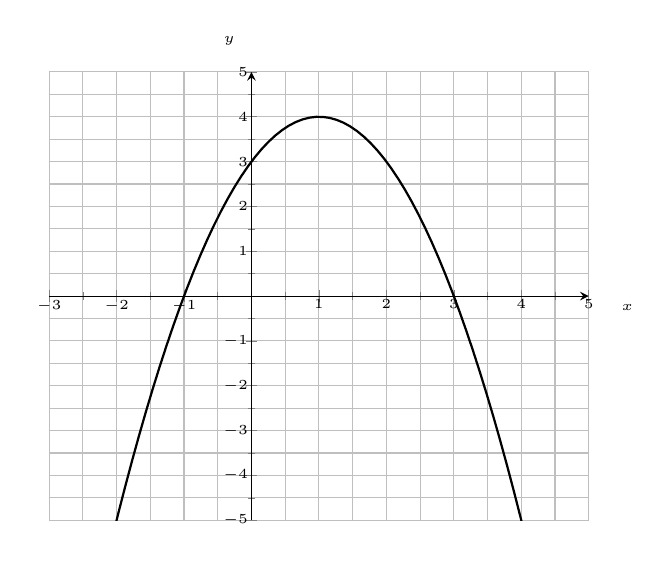
\begin{tikzpicture}[scale=1]
 \begin{axis}[grid=both, ymin=-5,ymax=5,xmax=5,xmin=-3,xtick={-3,-2,...,5},ytick={-5,-4,...,5},minor tick num=1, axis lines = middle,xlabel=$x$,ylabel=$y$, 
x tick label style={yshift=1ex,font={\tiny}}, y tick label style={xshift=1ex, font={\tiny}}, label style ={at={(ticklabel cs:1.1)}, font={\tiny}}
]
 \addplot[thick, samples=100]   {-(x-1)^2+4};                        
  \end{axis}
\end{tikzpicture}
\end{center}
\end{minipage}
\end{minipage}
\begin{solution}\mbox{}\\
\begin{enumerate*}[label={(\arabic*)},itemjoin=\qquad]
	\item $(-1, 3)$.
	\item $(-\infty, \infty)$.
	\item $(-\infty, 4]$
	\item $f(0)=3$.
\end{enumerate*}\\
\begin{enumerate*}[resume*]
	\item $(-1,0)$ and $(3,0)$.
	\item $(0, 3)$.
	\item $(1, 4)$.
	\item $x=0$ or $x=2$.
\end{enumerate*}
\end{solution}